%% LyX 1.1 created this file.  For more info, see http://www.lyx.org/.
%% Do not edit unless you really know what you are doing.
\documentclass[10pt,a4paper]{article}
\usepackage{times}
\usepackage{geometry}
\geometry{verbose,a4paper,tmargin=1.2in,bmargin=1.2in,lmargin=1in,rmargin=1in}
\usepackage{graphics}
\usepackage{verbatim}
\usepackage{graphicx}
%\usepackage{mathptm}
\usepackage{psfrag}
%\usepackage{subfigure}
\usepackage{subfig}
\usepackage{amsfonts}
\usepackage{longtable}
\usepackage{comment}
\usepackage{paralist}
\usepackage{color}
\usepackage{microtype}
\usepackage{cite}
\usepackage{tikz}
\usepackage{tikz-dependency}
\usepackage{url}
\usepackage{amsmath}
\usepackage{multirow}
\usepackage[shortlabels]{enumitem}

\newtheorem{definition}{Definition}
\newtheorem{example}{Example}
\newtheorem{algocounter}{Algorithm}[section]
\newtheorem{lemma}{Lemma}
\newtheorem{theorem}{Theorem}


\makeatletter

%%%%%%%%%%%%%%%%%%%%%%%%%%%%%% LyX specific LaTeX commands.
\providecommand{\LyX}{L\kern-.1667em\lower.25em\hbox{Y}\kern-.125emX\@}
%% Special footnote code from the package 'stblftnt.sty'
%% Author: Robin Fairbairns -- Last revised Dec 13 1996
\let\SF@@footnote\footnote
\def\footnote{\ifx\protect\@typeset@protect
    \expandafter\SF@@footnote
  \else
    \expandafter\SF@gobble@opt
  \fi
}
\expandafter\def\csname SF@gobble@opt \endcsname{\@ifnextchar[%]
  \SF@gobble@twobracket
  \@gobble
}
\edef\SF@gobble@opt{\noexpand\protect
  \expandafter\noexpand\csname SF@gobble@opt \endcsname}
\def\SF@gobble@twobracket[#1]#2{}

%%%%%%%%%%%%%%%%%%%%%%%%%%%%%% User specified LaTeX commands.
\newtheorem{Example}{Example}[section]
\newtheorem{Definition}{Definition }[section]
\usepackage{graphicx}

\makeatother
\begin{document}
\newcommand{\blue}[1]{\textcolor{blue}{#1}}
\newcommand{\green}[1]{\textcolor{green}{#1}}
\newcommand{\red}[1]{\textcolor{red}{#1}}


\title{\fontsize{18}{18} \textbf{{To be decided}}}

\date{{}}

\vspace{-3.0cm}

\maketitle
\thispagestyle{empty}


{\centering \fontsize{13}{13} \em Synopsis of the Thesis to be
submitted in Partial Fulfillment \par}

{\centering \fontsize{13}{13} \em of the Requirements for the
Award of the Degree of\par}


\vspace{1.0cm}

{\centering {\fontsize{14}{14} \textbf{Doctor of Philosophy}}\par}

\vspace{0.8cm}

{\centering \fontsize{13}{13} \em by\par}

\vspace{0.5cm}

{\centering {\fontsize{14}{14} \textbf{Abhijit Mondal}}\par}

\vspace{0.25cm}

{\centering {\fontsize{14}{14} \textbf{(15CS91R09)}}\par}

\vspace{1.0cm}

{\centering \fontsize{13}{13} \em Under the supervision of\par}

\vspace{0.6cm}

{\centering {\fontsize{14}{14} \textbf{Prof. Sandip Chakraborty}}\par}
% \vspace{0.25cm}
% {\centering {\fontsize{14}{14} \em and}\par}
% \vspace{0.25cm}
% {\centering {\fontsize{14}{14} \textbf{Prof. Partha Pratim Chakrabarti}}\par}

\vspace{1cm}

{\centering \resizebox*{!}{4.0cm}{
\includegraphics{img/iit_kgp_logo.png}}
\par}

\vspace{1.0cm}

{\centering {\fontsize{14}{14} \textbf{Department of Computer
Science and Engineering}}\par}

% \vspace{0.5cm}

{\centering {\fontsize{14}{14} \textbf{Indian Institute of
Technology Kharagpur}}\par}

\vspace{0.2cm}

{\centering {\fontsize{14}{14} \textbf{March 2020}}\par}

\newpage
\thispagestyle{empty} \vspace*{2cm} \newpage
\tableofcontents
\thispagestyle{empty}
\newpage
\thispagestyle{empty} \vspace*{2cm} \newpage
\parskip 0.1in
\setcounter{page}{1}
%===========================================
%           report
%===========================================
%\input{report}
%\section{Introduction}
Online video streaming is the most popular service on the Internet. The pervasive penetration of smartphone and availability of cheap LTE network make it even easier for reach to millions of users.
%The introduction of the video streaming system over the HTTP and in build player in HTML5 makes it easier to start a new video streaming service on the one hand. On the other hand, the LTE network's pervasive penetration makes it easier for smartphone users to watch online videos. On top of HTTP and HTML5, dynamic adaptation of the audio-video quality allows stream providers to make the service tolerant to frequent network change. These technologies gain the attention of researchers all around the globe. In this work, we discuss the technological advancement for video streaming using HTTP.
Video streaming can be primarily categorized into three categories: i) static video or video-on-demand (VoD) streaming, ii) live video streaming, and iii) interactive video streaming. Video streaming services like YouTube, NetFlix, Prime videos fall into the video-on-demand category. Here the videos are prerecorded and preprocessed. YouTube-Live, Periscope, Twitch provide live video streaming Category. The only difference between VoD and live video streaming is that videos are not preprocessed in live streaming as it is not ready yet. The services like video conferencing, webinars are fall in the third category, the interactive video. The interactive online videos are not only bidirectional but also extremely delay-sensitive. Unlike VoD or live streaming, it is okay for interactive video streaming to drop several frames than stall for data. So, the technology required for the interactive video is very different in every aspect. In our work, we concentrated on the VoD and live video streaming over HTTP only.

HTTP is a widely accepted protocol as it serves the World-Wide-Web (WWW). Most of the firewalls, proxies, and NAT-boxes allow HTTP protocol. HTTPS, the secure version of HTTP, is equally acceptable for the network administrator of different organizations. So, the HTTP(S) based video streaming services also allowed by those firewalls, proxies, and NAT boxes. This one feature favored HTTP(S) based video streaming over the existing video streaming system.

On top of the HTTP-based video streaming system, service providers can now adapt video quality according to the available network quality. It reduces the rebuffering significantly. Currently, most online video services support adaptive video streaming as it provides a better quality of experience to the viewers. Several technologies like MPEG-DASH (dynamic adaptive streaming over HTTP), Apple's HLS, and SmoothStream by Microsoft developed to provide dynamic adaptive streaming. Although different organizations develop these technologies, they work almost identically. In our work, we concentrate on the DASH only as it is a guideline than a product and the open-source implementation of DASH is available.

DASH or DASH-like video streaming systems changes video quality on the fly running a special algorithm call adaptive bitrate algorithm (ABR). The selection of ABR is crucial as the overall quality of experience is dependent on this algorithm. It is the ABR algorithms' job to provide minimal rebuffering while maintaining better video quality. In our survey, we first discuss the details of the DASH and different components of DASH. We then discuss DASH's application on YouTube, a major video streaming provider, and the latest research on the ABR to provide better QoE for both VoD and live streaming in different scenarios.

%\subsection{DASH}
%
%%
%Dynamic Adaptive Streaming over HTTP (DASH), also referred to as MPEG-DASH, is an adaptive bit-rate solution for video streaming, which enables client-operated video delivery over HTTP.
%%
%DASH is implemented by breaking down the video content into small segments, each worth a short duration of playback time.
%%
%For every segment of playback time, alternative versions at various bit-rates are available at the server.
%%
%The client typically requests for the highest quality segment possible under current network conditions, such that it is received (downloaded) in time for playback, without causing stalling or re-buffering. 
%%
%However, DASH is not a protocol -- it only specifies an architecture (Fig.~\ref{fig:dash}) to enable adaptive video streaming over HTTP.
%%
%Every video streaming service (e.g., YouTube, Netflix, etc.) is free to define its own implementation of the DASH modules.
%
%\subsection{ABR}
%Adaptive bitrate algorithm or ABR algorithm is the heart of the DASH. ABR decide when and which quality to download based on network quality and other parameter. Primary job of any ABR algorithm is improve user experience by selecting appropriate video quality for the a segment. As the online video streaming become one of the most popular service in the Internet, it become more prevalent to improve ABR algorithm to provide better QoE in different. The problem attract researcher from academic as well as the industries. Researcher start exploiting different areas of video streaming with a common goal, i.e. improving QoE for end user.
%
%\subsection{QoE}
%Quality of Experience is a important parameter in any field which involves end users. In case of the video streaming, QoE is metric to measure whether user have enjoyed the video or not. QoE is mostly a user perspective and it depends on several factor such as startup delay, quality flactuation, overall quality, rebuffering, audio/video device, video content. Although all this parameters are important, it is difficult to measure user dependent parameter and video content. Several researcher tried to to find best measurable metric to calculate QoE which can be acceptable. Mok \etal \cite{5990550} tried to calculate QoE from the network QoS. Infact they suggested that user QoS (or QoS of HTTP) is the QoE. 
%
%\blue{TODO: More about QoE}

\section{Adaptive Bitrate Streaming over Today’s Internet: A Case Study of YouTube}
We analyze the YouTube video streaming system to explore the interplay among various parameters that impact the ABR decision. Although YouTube follows DASH guidelines, it deviates a lot from it. For example, it does not use the standard MPD file; instead, it uses a self-defined format. Similarly, there are several optimizations, and parameters are not known. We collect traffic traces of a sizable amount of YouTube video via a controlled environment and identify the unknown optimizations and parameters.
\subsection{Experimental setup}
In our experiment, we target web-based YouTube player as the data collection platform. Our goal is to collect the HTTP Archive (HAR) of a video session that is available in the debug tool of browsers and {\tt tcpdump} trace. We also want to control the network speed while playing video to understand the quality adjustment triggering point. We automate this entire setup using 3 tools, a) custom build throttler using the Linux library {\tt NetFilterQueue}, c) Firefox plugin {\tt har\_export\_trigger} (version 0.5.0-beta) to dump the HAR automatically without user intervention, and b) {\tt Selenium} to automate the video playback and trigger HAR export. Using our throttler, we change the bandwidth from 200kbps to 2400kbps with a step of 200kbps.
\subsection{Observations}
\subsubsection{Parameter identification}
We find that YouTube forwards several parameters to the server with each HTTP request to fetch the video data from the collected traces. Among these parameters we find {\tt rbuf} and {\tt range} particularly interesting. The {\tt rbuf} is the remaining buffer for a particular {\tt itag} and {\tt range} is data segment (in bytes) of the full video of the particular {\tt itag}. From {\tt range},  we identify the video segment length (in seconds) requested in a HTTP request. We utilize these observations for further analysis.
\subsubsection{Insights into YouTube’s Bitrate Adaptation Algorithm}
With the help of identified parameters, we understand the adaptation strategy up to a certain degree. We find that YouTube takes an opportunistic approach to upgrade video quality when link quality goes up and takes a conservative approach to downgrade video quality while network quality drops. We also find that YouTube adapts segment length as per the network quality. When it finds a steady network condition, it increases the segment length and decreases when it finds poor network conditions.
\subsubsection{Data wastage}
Segment length adaptation may have far-reaching implications in terms of advantages for YouTube streaming, one of which is minimal data wastage. Since segment length increases gradually from lower values to higher values when bandwidth improves, overlaps between the segments of a lower quality and the next higher quality are largely diminished. This implies that data wastage values come down drastically (as opposed to a scenario with no segment length adaptation) – in our experiments, we compute the average wastage ratio, defined as $\frac{data\_downloaded - data\_played}{data\_played}$, to be $0.82\times10^{-6}$. This is in sharp contrast with previously reported values.

\section{Transport Protocols and Mobility Choices for ABR Streaming: Performance vs Energy Efficiency}
Any ABR take decision based on the directly or indirectly observed network throughput. However, this throughput is highly depends on the underlying transport protocol QUIC or TCP. As all the ABR algorithms are primarily designed with TCP in the mind, we want to know if those existing ABR algorithm can work fine with the QUIC or other set of algorithms are required. On the other hand, the performance of an ABR algorithm can indirectly impact the power consumption of smartphones due to the nature of the radio resource controller (RRC).

\subsection{TCP vs QUIC: YouTube}
YouTube started using QUIC as an alternative to TCP via Google chrome and chromium browser. Both of these browser support flag to enable or disable QUIC during run time. So we run player ~175 videos by enabling and disabling the QUIC and record the HAR and {\tt tcpdump} trace. 
\subsubsection{Observation}
We want to know QUIC provide better quality than TCP or not. So, we look for the three parameters rebuffering, average quality and quality switches in our collected traces. We find that QUIC incurs less quality switches than TCP and over all quality is better with QUIC than the TCP. In terms of rebuffering we find interesting results. When network quality is very poor, QUIC suffers more than the TCP. However, TCP suffers more when network quality is better.

\subsection{TCP vs QUIC: DASH}
We compare performance of modern ABRs like BOLA, MPC, and Pensieve between QUIC and TCP. For the experiment purpose, we use the open source DASH-IF player and publicly available network trace to throttle the connection with the help of {\tt mahimahi} tool. We keep the server and the experimental client in the same network and throttle the connection using {\tt mahimahi}. In this experiment we played approx 50 videos of total 45 hours playback time using various ABR algorithm.

\subsubsection{Observation}
Our initial observations showed that the QUIC is performing poorly for all most all the scenarios in term of all the QoE components and the over all QoE for most of the scenarios. Fig.~\ref{fig:chap03s2:RebufferTime_n} and Fig.~\ref{fig:chap03s2:QOE_n} depict the observations on rebuffering and QoE.
\begin{figure*}[!h]
%	\begin{minipage}[t]{0.48\linewidth}
%		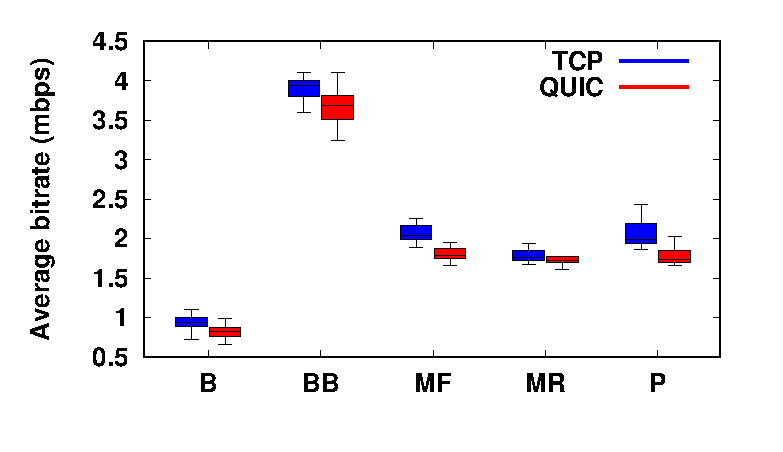
\includegraphics[width=\linewidth]{img/QUIC/bitrate_box}
%		\caption{\label{fig:chap03s2:averageQuality_n}Average Playback Video Quality for Different ABR Techniques ($p<0.05$ for all the metrics)}
%	\end{minipage}\hfill
%	\begin{minipage}[t]{0.48\linewidth}
%		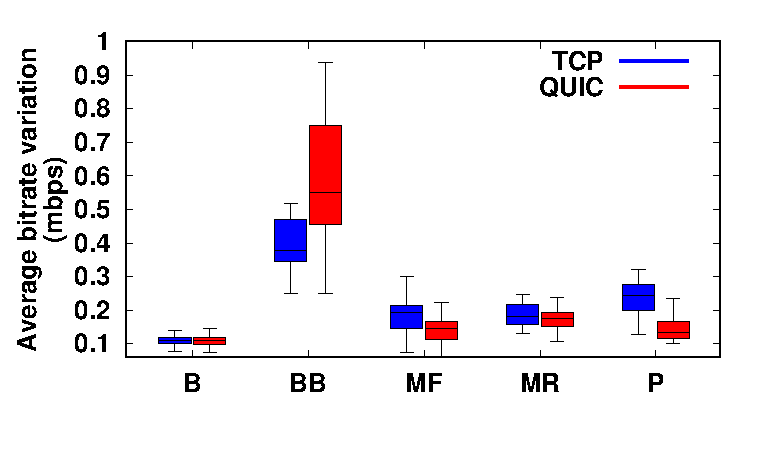
\includegraphics[width=\linewidth]{img/QUIC/smooth_box}
%		\caption{\label{fig:chap03s2:averageQualityVariation_n}Average Playback Quality Variation for Different ABR Techniques ($p<0.05$ for all the metrics except BOLA and MPC-Robust)}
%	\end{minipage}
%	
	\begin{minipage}[t]{0.48\linewidth}
		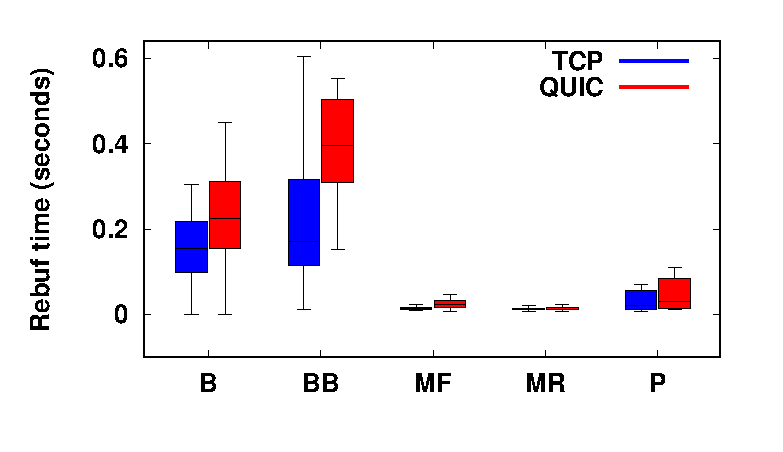
\includegraphics[width=\linewidth]{img/QUIC/rebuf_box}
		\caption{\label{fig:chap03s2:RebufferTime_n}Rebuffering Time for Different ABR Techniques ($p<0.05$ for all the metrics except Pensieve and MPC-Robust)}
	\end{minipage}\hfill
	\begin{minipage}[t]{0.48\linewidth}
		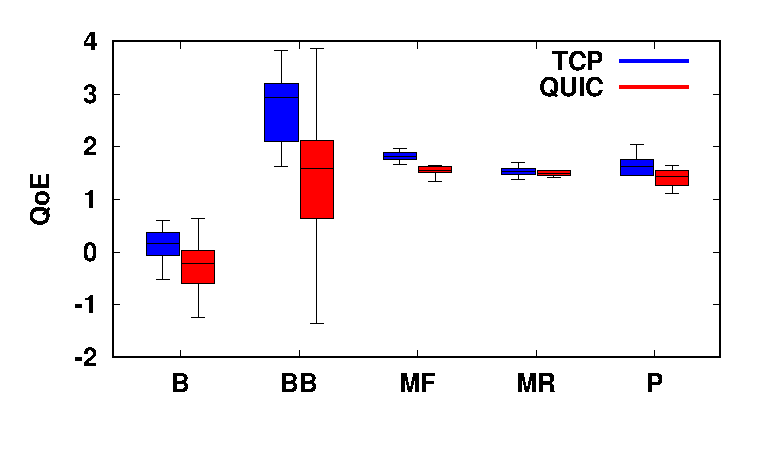
\includegraphics[width=\linewidth]{img/QUIC/qoe_box}
		\caption{\label{fig:chap03s2:QOE_n}Overall QoE for Different ABR Techniques ($p<0.05$ for all the metrics except MPC-Robust)}
	\end{minipage}
\end{figure*}
\section{EnDASH - A Mobility Adapted Energy Efficient ABR Video Streaming for Cellular Networks}
From the observations in previous sections, we design an ABR algorithm, EnDASH, which aims to reduce the radio's energy consumption during the video streaming. EnDASH reads the environment by means of different parameters and try to predict the future. Based on the prediction, it schedules segment downloading in a way so that it reduces energy consumption. It does not directly schedule it. Instead, it changes the available buffer (which is a parameter) in the player, and DASH it self schedule the segment downloading according to the buffer.
\subsection{EnDASH System}
The EnDASH first predicts an expected throughput for the short future ($t$) from the past, and based on predicted throughput, it decides the buffer length for $t$ duration. Later on, it also decides the bitrate based on the past information and current buffer length, and predicted throughput. EnDASH use three machine learning engine for each step.

\begin{figure}[!h]
	\centering
	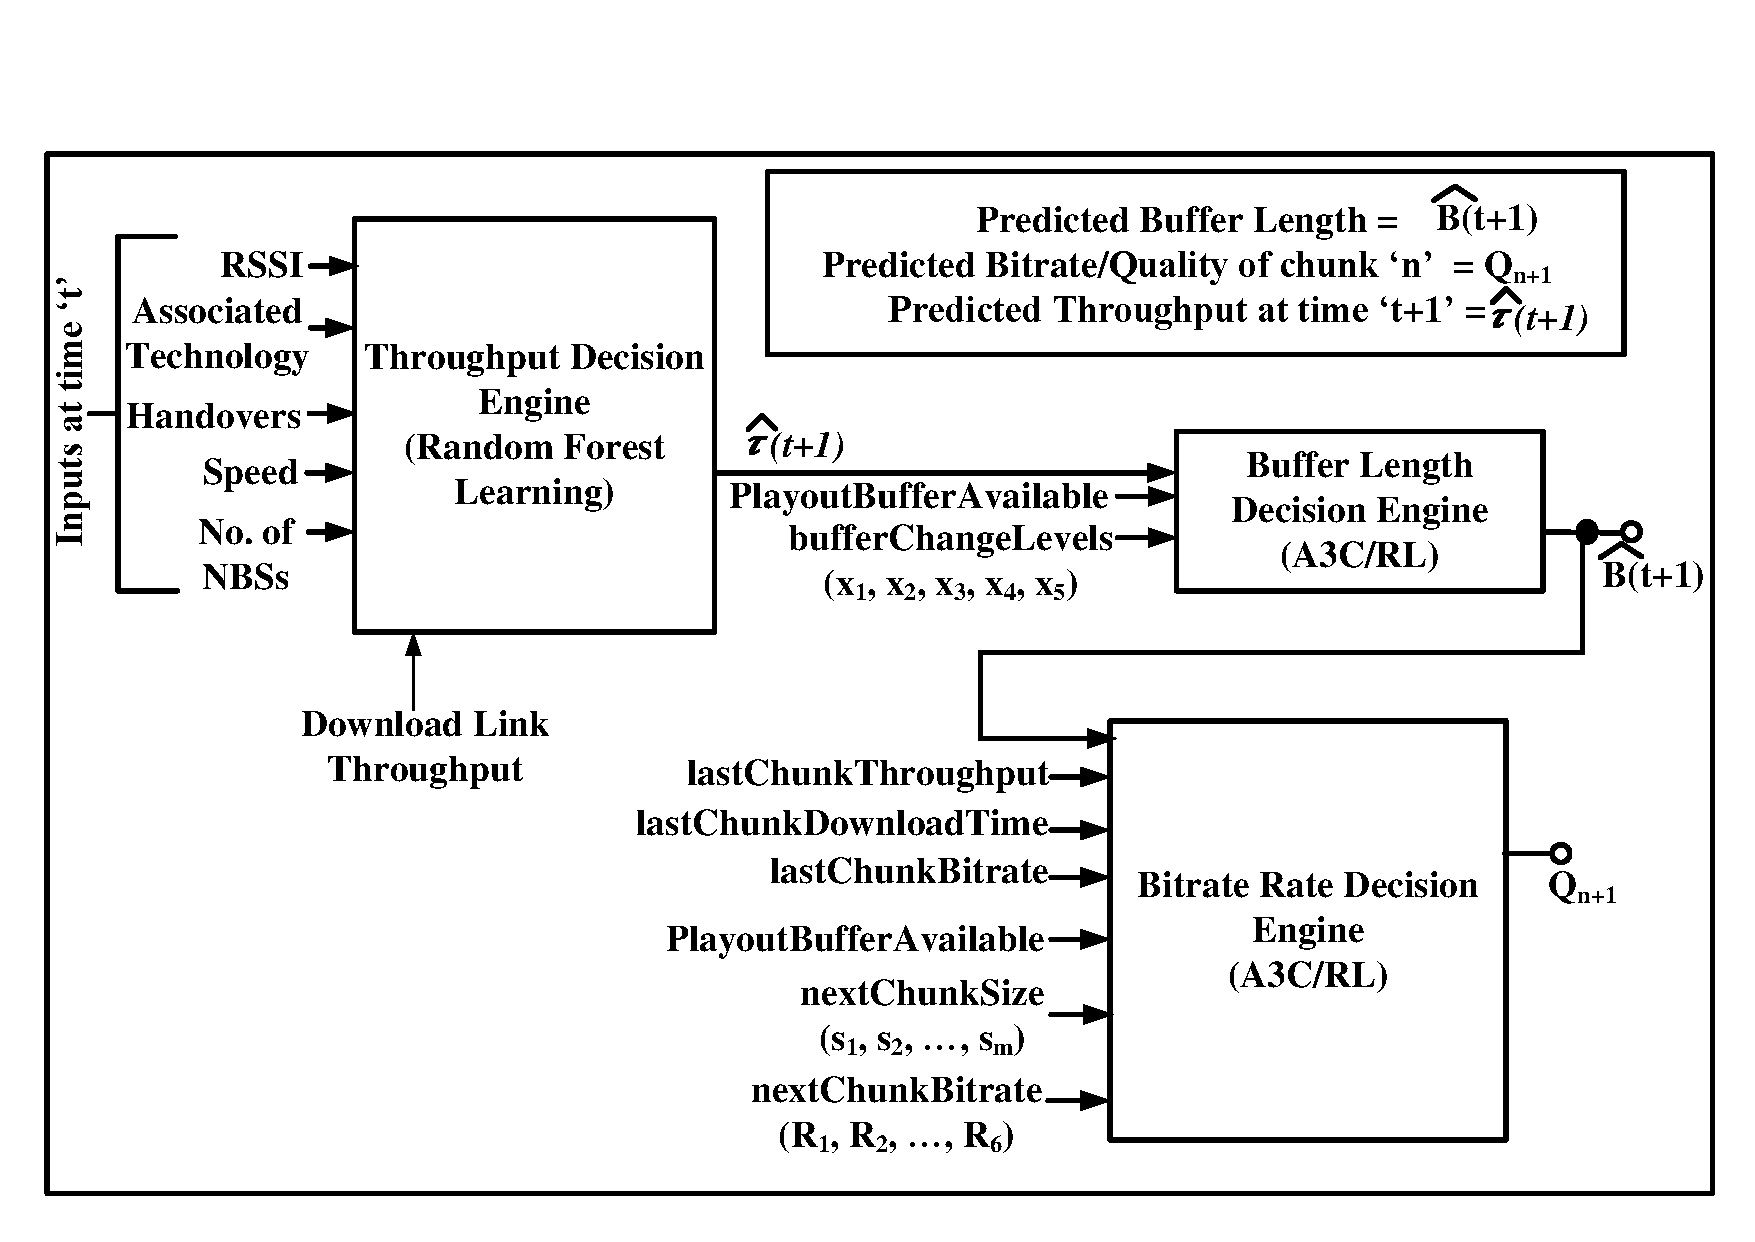
\includegraphics[width=0.7\linewidth]{img/EnDASH/EnDASH_system}
	\caption{Composite Representation of the EnDASH model; a cascaded model where the predicted throughput acts as an input network state to the Actor Critic RL based decision
engine}
	\label{fig:endash:system}
\end{figure}

\subsubsection{The throughput prediction engine}
EnDASH uses random forest learning to predict expected throughput for the next 30sec from past information. It uses features like device's speed, cellular RSSI, current technology, handovers. As the features sets are huge, we feed only the $\mathrm{25^{th}}$, $\mathrm{75^{th}}$, and $\mathrm{90^{th}}$ percentile points, median and mean from its historical data of each feature.
\subsubsection{The Buffer Length Decision Engine}
The buffer length decision engine uses an A3C RL based deep neural network to determine the optimal buffer length. It takes the predicted throughput, last buffer length, and possible steps to change buffer length. It returns the decision whether buffer length needs to increase or decrease or keep the same. We use a linear weighted function of energy savings during the training phase with respect to a baseline ABR algorithm and the QoE score as the reward.

The throughput prediction engine and buffer length prediction engine runs only once every $t$ time and in these order only.

\subsubsection{The Bitrate Decision Engine}
EnDASH use another A3C RL based deep neural network on estimating the quality of the next chunk based on several playbacks related players and the buffer length similar to the parameters used in the Pensieve\cite{mao2017neural}. It runs before fetching the next segment and uses QoE as the reward during the training phase.

The complete architecture of the EnDASH decision engines is presented in the Fig.~\ref{fig:endash:system}.

\begin{figure}[!h]
	\begin{minipage}[t]{0.48\linewidth}
		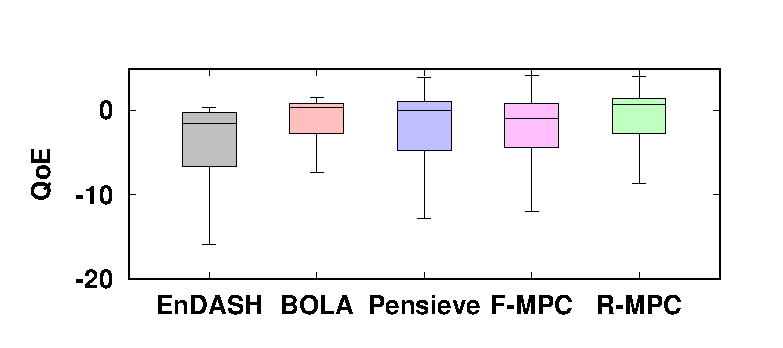
\includegraphics[width=\linewidth]{img/EnDASH/QoE}
		\caption{\label{fig:endash:qoe}}
	\end{minipage}\hfill
	\begin{minipage}[t]{0.48\linewidth}
		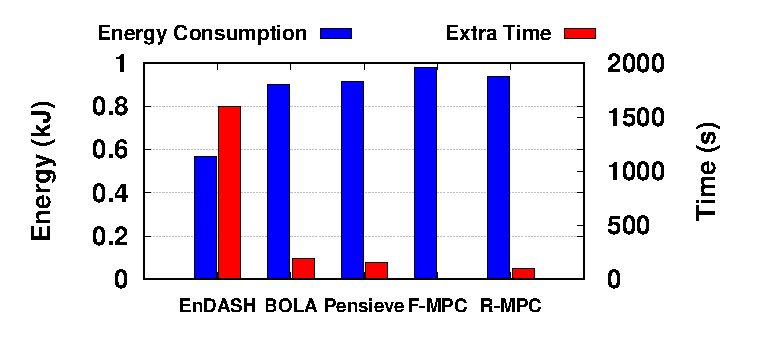
\includegraphics[width=\linewidth]{img/EnDASH/EnergyConsumption}
		\caption{\label{fig:endash:energy}}
	\end{minipage}
\end{figure}
\subsection{Evaluation}
We trained and tested all these three engines in an emulation platform with the data we collected from commodity smartphones like Moto G5, Micromax canvas over Airtel, Reliance Jio, and Vodaphone. Once training and testing are completed for each individual module, we run experiments in our emulation based testbed, comparing QoE performance and energy saving of EnDASH. In Fig.~\ref{fig:endash:qoe} we compare the performance in terms of QoE with modern ABR algorithms. EnDASH slightly compromises the QoE; however, it saves a lot of energy. In Fig.~\ref{fig:endash:energy}, we plot the energy uses and possible run time with respect to Fast-MPC, and it turns out that video can be played for another 20-25 minutes with EnDASH compared to Fast-MPC.

\section{Federated Adaptive Bitrate Live Streaming over Locality Sensitive Playback Coalitions}
\red{Live streaming is a unique service in the Internet which is alternative to TV broadcast yet more flexible. Few live streaming provider allow ability add custom delay. However, most popular flavor of live streaming is without any user defined delays. The live stream have a unique property of synchronous playback by millions of players. In case of mega event, we find another interesting property that many player belongs same local networks. There is two special case exists a) Internet on cable where users have different connection even though they are connected via local networks, b) shared Internet connection where multiple user/player share same Intenet backbone. We want to develop a DASH based live streaming system where players forms coalition if they are connected via local network and stream the live video as a group. Incase of large network, Application-Layer Traffic Optimization (ALTO) server will be use to find appropriate players. Our goal is to improve quality }
%======================
\section{Organization of the Thesis}

In this section, we provide a brief description of the organization of the thesis.
\begin{itemize}
	\item {\bf Chapter 1} introduces the thesis with background, motivation, objectives, and scope of the thesis.
	\item {\bf Chapter 2} provides the details of online video streaming system and different ABR algorithms developed in the past. Moreover, it iterates over the merits and demerits of the proposed solution to the problem broadly linked with this thesis.
	\item {\bf Chapter 3} presents the study on YouTube video streaming service and analyses the adaptation technique taken by YouTube.
	\item {\bf Chapter 3} performs a study to analyze the performance difference between two transport protocols, TCP and QUIC, on the adaptive bitrate video streaming system, with both YouTube and standard DASH player from DASH Industry Forum. We further analyze the energy consumption by a smartphone during online video streaming in various mobility scenarios.
	\item {\bf Chapter 4} presents a novel ABR algorithm, called EnDASH, to reduce the energy consumption during the online streaming by optimizing the segmented schedule in buffer length.
	\item {\bf Chapter 5} proposes a DASH-based live video streaming system which exploits the locality information to improve the video QoE and decreases the network usage by sharing segment among local players. It also describes a novel approach to form a coalition among the local players and decides the bitrate for the entire coalition.
	\item {\bf Chapter 7} concludes the thesis by summarizing our contributions and listing down the possible future directions.
\end{itemize}
\section{Conclusion}
This report provided a broad summary of the thesis having four contributory chapters dealing with analyzing and optimizing video streaming services over the Internet. Our first contributory chapter deals with analyzing the YouTube ABR mechanism and with finding out various parameters that impact YouTube streaming at large. The second contributory chapter explores the impact of protocol choice and mobility on ABR performance. Based on these analyses, the third contributory chapter develops an energy-efficient streaming algorithm for the Internet. The final contributory chapter discusses the design of an adaptive live streaming platform by exploring the ALTO service. In a nutshell, this thesis enriches the current literature from two different aspects. First, it thoroughly analyzes the current ABR techniques over popular OTT media services like YouTube and opens up various problems and challenges associated with it. Second, it proposes two optimizations over the current streaming media protocols, one in the direction of supporting energy efficiency during VoD streaming over smartphones, and the other in developing an efficient mechanism for adaptive live streaming.

Although this thesis solves a few challenges associated with scaling up video streaming services over the Internet, there are many open problems that can be taken up as future research directions in this area. First, we have shown the current ABR techniques do not work well with QUIC and highlighted the reasons behind that. Therefore, efficient protocols can build up the synergy among the application layer streaming services and the underlying network protocol. Second, the practical implementation of ML and DL-based ABR techniques is still an open problem. Necessary architectural changes need to be designed to support the ML and DL-based ABR techniques over the client devices. Third, innovative methods like super-resolution have been proposed in the literature. It will be interesting to check how these modern techniques work over the existing ABR algorithms. 
\section{Publications out of the Thesis}
\subsection{Journal}
\begin{enumerate}[start=1,label={[\arabic*]}]
	\item \textbf{Abhijit Mondal}, Sandip Chakraborty, ``\textit{Does QUIC Suit Well with Modern Adaptive Bitrate Streaming Techniques?}”, in IEEE Networking Letters, vol. 2, no. 2, pp. 85-89, June 2020.
\end{enumerate}
\subsection{Conference and Workshop Proceedings}
\begin{enumerate}[start=1,label={[\arabic*]}]
	\item \textbf{Abhijit Mondal}, Sandip Chakraborty, ``\textit{Federated Adaptive Bitrate Live Streaming over Locality Sensitive Playback Coalitions}”, in proceedings of the ACM SIGCOMM Workshop on Network Application Integration/CoDesign (ACM SIGCOMM NAI '20), Association for Computing Machinery, New York, USA, August 11 - 14, 2020. 
	\item \textbf{Abhijit Mondal}, Basabdatta Palit, Somesh Khandelia, Nibir Pal, Jay Jayatheerthan, Krishna Paul, Niloy Ganguly and Sandip Chakraborty, ``\textit{EnDASH - A Mobility Adapted Energy Efficient ABR Video Streaming for Cellular Networks}'', in the proceedings of the 2020 IFIP Networking Conference (IFIP Networking), Paris, France, June 22-25, 2020.
	\item \textbf{Abhijit Mondal}, Satadal Sengupta, B.R. Reddy, M.J.V. Koundinya, Chander G., Pradipta De, Niloy Ganguly, Sandip Chakraborty, ``\textit{Candid with YouTube: Adaptive Streaming Behavior and Implications on Data Consumption}'' in Proceedings of the 27th Workshop on Network and Operating Systems Support for Digital Audio and Video (ACM NOSSDAV’17), Taipei, Taiwan, June 20 - 23, 2017.
\end{enumerate}

\footnotesize
\bibliographystyle{ieeetr}
\addcontentsline{toc}{section}{\numberline{}References}
\bibliography{ref/thesis,ref/collection,ref/others}
\end{document}
